\documentclass[aspectratio=169]{beamer}

% --- THEME AND STYLING ---
\usetheme{Madrid}
\useoutertheme{default}
\useinnertheme{rectangles}
\setbeamertemplate{navigation symbols}{}

% --- CUSTOM COLOR PALETTE ---
\definecolor{SkyBlue}{RGB}{135, 206, 235}
\definecolor{DarkNavy}{RGB}{0, 0, 139}
\definecolor{LightBlueBg}{RGB}{240, 248, 255}
\definecolor{AccentBlue}{RGB}{70, 130, 180}
\definecolor{DarkGreyText}{RGB}{50, 50, 50}
\definecolor{HighlightGreen}{RGB}{34, 139, 34}
\definecolor{AlertRed}{RGB}{220, 20, 60}

\setbeamercolor{palette primary}{bg=SkyBlue,fg=DarkNavy}
\setbeamercolor{palette secondary}{bg=DarkNavy,fg=white}
\setbeamercolor{palette tertiary}{bg=AccentBlue,fg=white}
\setbeamercolor{palette quaternary}{bg=SkyBlue,fg=DarkNavy}
\setbeamercolor{structure}{fg=DarkNavy}
\setbeamercolor{section in toc}{fg=DarkNavy}
\setbeamercolor{frametitle}{bg=SkyBlue,fg=DarkNavy}
\setbeamercolor{block title}{bg=DarkNavy,fg=white}
\setbeamercolor{block body}{bg=LightBlueBg,fg=DarkGreyText}
\setbeamercolor{block title alerted}{bg=AlertRed,fg=white}
\setbeamercolor{block body alerted}{bg=LightBlueBg,fg=DarkGreyText}
\setbeamercolor{block title example}{bg=HighlightGreen,fg=white}
\setbeamercolor{block body example}{bg=LightBlueBg,fg=DarkGreyText}
\setbeamertemplate{footline}[frame number]
\setbeamercolor{footline}{fg=DarkNavy}
\setbeamertemplate{blocks}[rounded][shadow=false]

% --- PACKAGES ---
\usepackage[utf8]{inputenc}
\usepackage{amsmath,amssymb}
\usepackage{booktabs}
\usepackage{graphicx}
\usepackage{array}
\usepackage{multirow}
\usepackage{tikz}
\usetikzlibrary{shapes,arrows,positioning,calc}
\usepackage{siunitx}

% --- TITLE PAGE ---
\title[Sustainable Rendezvous]{Sustainable "Rendezvous": A Festival Systems Challenge}
\subtitle{Module 3.1: Quantifying Environmental Load}
\author[Team Sustainability]{Sustainability Task Force}
\institute{Department of Chemical Engineering\\
\vspace{0.2cm}
\small Course: CLL782 - Process Optimization\\
\small Instructor: Prof. Om Prakash}
\date{\today}

\begin{document}

% --- TITLE SLIDE ---
\begin{frame}[plain]
    \titlepage
    \vspace{-0.5cm}
    \begin{center}
        \small Presented by: [Your Name/Team]
    \end{center}
\end{frame}

% --- OUTLINE ---
\begin{frame}{Outline}
    \tableofcontents[hideallsubsections]
\end{frame}

%%%%%%%%%%%%%%%%%%%%%%%%%%%%%%%%%%%%%%%%%%%%%%%%%%%%%%%%%%%%%%%%%
\section{Problem Statement \& Introduction}
%%%%%%%%%%%%%%%%%%%%%%%%%%%%%%%%%%%%%%%%%%%%%%%%%%%%%%%%%%%%%%%%%

\begin{frame}{The Challenge: Greening Asia's Largest Fest}
    \begin{columns}[T]
        \begin{column}{0.55\textwidth}
            \begin{block}{Context}
                \begin{itemize}
                    \item \textbf{Rendezvous (IIT Delhi)}: $\sim$160,000 attendees over 4 days.
                    \item A celebration of culture, art, and talent.
                    \item \textbf{The Hidden Cost}: Massive environmental footprint (Waste, Energy, Carbon).
                \end{itemize}
            \end{block}

            \begin{alertblock}{The Objective}
                Transform Rendezvous into a \textbf{model of sustainability} by using Process Optimization to:
                \begin{itemize}
                    \item Quantify Environmental Load ($E$).
                    \item Optimize Infrastructure ($S, A$).
                    \item Plan Logistics (Bins, Water, Transport).
                \end{itemize}
            \end{alertblock}
        \end{column}

        \begin{column}{0.40\textwidth}
            \begin{exampleblock}{Vision}
                \textit{"Sustainability is not about restriction, but about acting responsibly and optimizing resources."}
                
                \vspace{0.2cm}
                \textbf{Goal:} Minimize Ecological Footprint while maximizing Festival Value.
            \end{exampleblock}
        \end{column}
    \end{columns}
\end{frame}

%%%%%%%%%%%%%%%%%%%%%%%%%%%%%%%%%%%%%%%%%%%%%%%%%%%%%%%%%%%%%%%%%
\section{Module 3.1: Modeling Environmental Load}
%%%%%%%%%%%%%%%%%%%%%%%%%%%%%%%%%%%%%%%%%%%%%%%%%%%%%%%%%%%%%%%%%

\begin{frame}{Methodology: The Environmental Load Function}
    \begin{block}{Defining the Objective Function}
        We define Total Environmental Load, $E$, as a function of key decision variables:
        $$ E(N, S, A) = E_{base} + E_{scale} + E_{inter} $$
    \end{block}

    \begin{columns}[T]
        \begin{column}{0.48\textwidth}
            \textbf{Variables:}
            \begin{itemize}
                \item $N$: Number of Attendees (Demand)
                \item $S$: Number of Stalls (Service Infrastructure)
                \item $A$: Activity Hours (Value Generation)
            \end{itemize}
        \end{column}
        \begin{column}{0.48\textwidth}
            \textbf{Components:}
            \begin{itemize}
                \item \textbf{Energy}: Grid/Diesel usage ($\epsilon$)
                \item \textbf{Waste}: Generated + Unsegregated
                \item \textbf{Emissions}: Transport + Operations
            \end{itemize}
        \end{column}
    \end{columns}
\end{frame}

\begin{frame}{Mathematical Formulation}
    \begin{alertblock}{The Model}
        \begin{equation*}
            E = \underbrace{(\alpha_1 N + \alpha_2 S + \alpha_3 A)}_{\text{Linear Base Load}} + 
                \underbrace{(\beta_N N^{1.3} + \beta_S S^{1.2} + \beta_A A^{0.8})}_{\text{Nonlinear Scale Effects}} + 
                \underbrace{\left( \gamma_{NS} \frac{N^2}{S} \right)}_{\text{Congestion Penalty}}
        \end{equation*}
    \end{alertblock}

    \vspace{0.2cm}
    \begin{itemize}
        \item \textbf{Diseconomies of Scale ($N^{1.3}$)}: Crowding leads to superlinear waste generation (littering, inefficiency).
        \item \textbf{Economies of Scale ($A^{0.8}$)}: Centralized infrastructure becomes more efficient.
        \item \textbf{Congestion Penalty ($N^2/S$)}: The critical term.
            \begin{itemize}
                \item If $S$ is too low (few stalls) $\rightarrow$ Long queues $\rightarrow$ Littering \& Chaos.
                \item If $S$ is too high $\rightarrow$ Wasted embodied energy ($\alpha_2 S$).
            \end{itemize}
    \end{itemize}
\end{frame}

\begin{frame}{Parameter Estimation for IIT Delhi}
    \begin{table}
        \caption{Estimated Parameters for Rendezvous Scenario}
        \centering\small
        \begin{tabular}{lcl}
            \toprule
            \textbf{Parameter} & \textbf{Value} & \textbf{Significance} \\ \midrule
            Attendees ($N$) & 160,000 & Total over 4 days \\
            Base Impact ($\alpha_1$) & 2.5 kg CO$_2$/p & Direct consumption \\
            Stall Impact ($\alpha_2$) & 18 kg CO$_2$/stall & Embodied energy + ops \\
            Crowding Exp ($\beta_N$) & 1.3 & Urban scaling law \\
            Congestion ($\gamma_{NS}$) & 0.0005 & Waste leakage factor \\
            \bottomrule
        \end{tabular}
    \end{table}

    \begin{exampleblock}{The Trade-Off}
        Optimization reveals a critical balance: we need enough stalls to prevent the $N^2/S$ congestion penalty from exploding, but not so many that $\alpha_2 S$ becomes wasteful.
    \end{exampleblock}
\end{frame}

%%%%%%%%%%%%%%%%%%%%%%%%%%%%%%%%%%%%%%%%%%%%%%%%%%%%%%%%%%%%%%%%%
\section{Region of Interest (ROI) Analysis}
%%%%%%%%%%%%%%%%%%%%%%%%%%%%%%%%%%%%%%%%%%%%%%%%%%%%%%%%%%%%%%%%%

\begin{frame}{Region of Interest (ROI) Mapping}
    \begin{columns}[T]
        \begin{column}{0.60\textwidth}
             % Including the map image using relative path
            \centering
            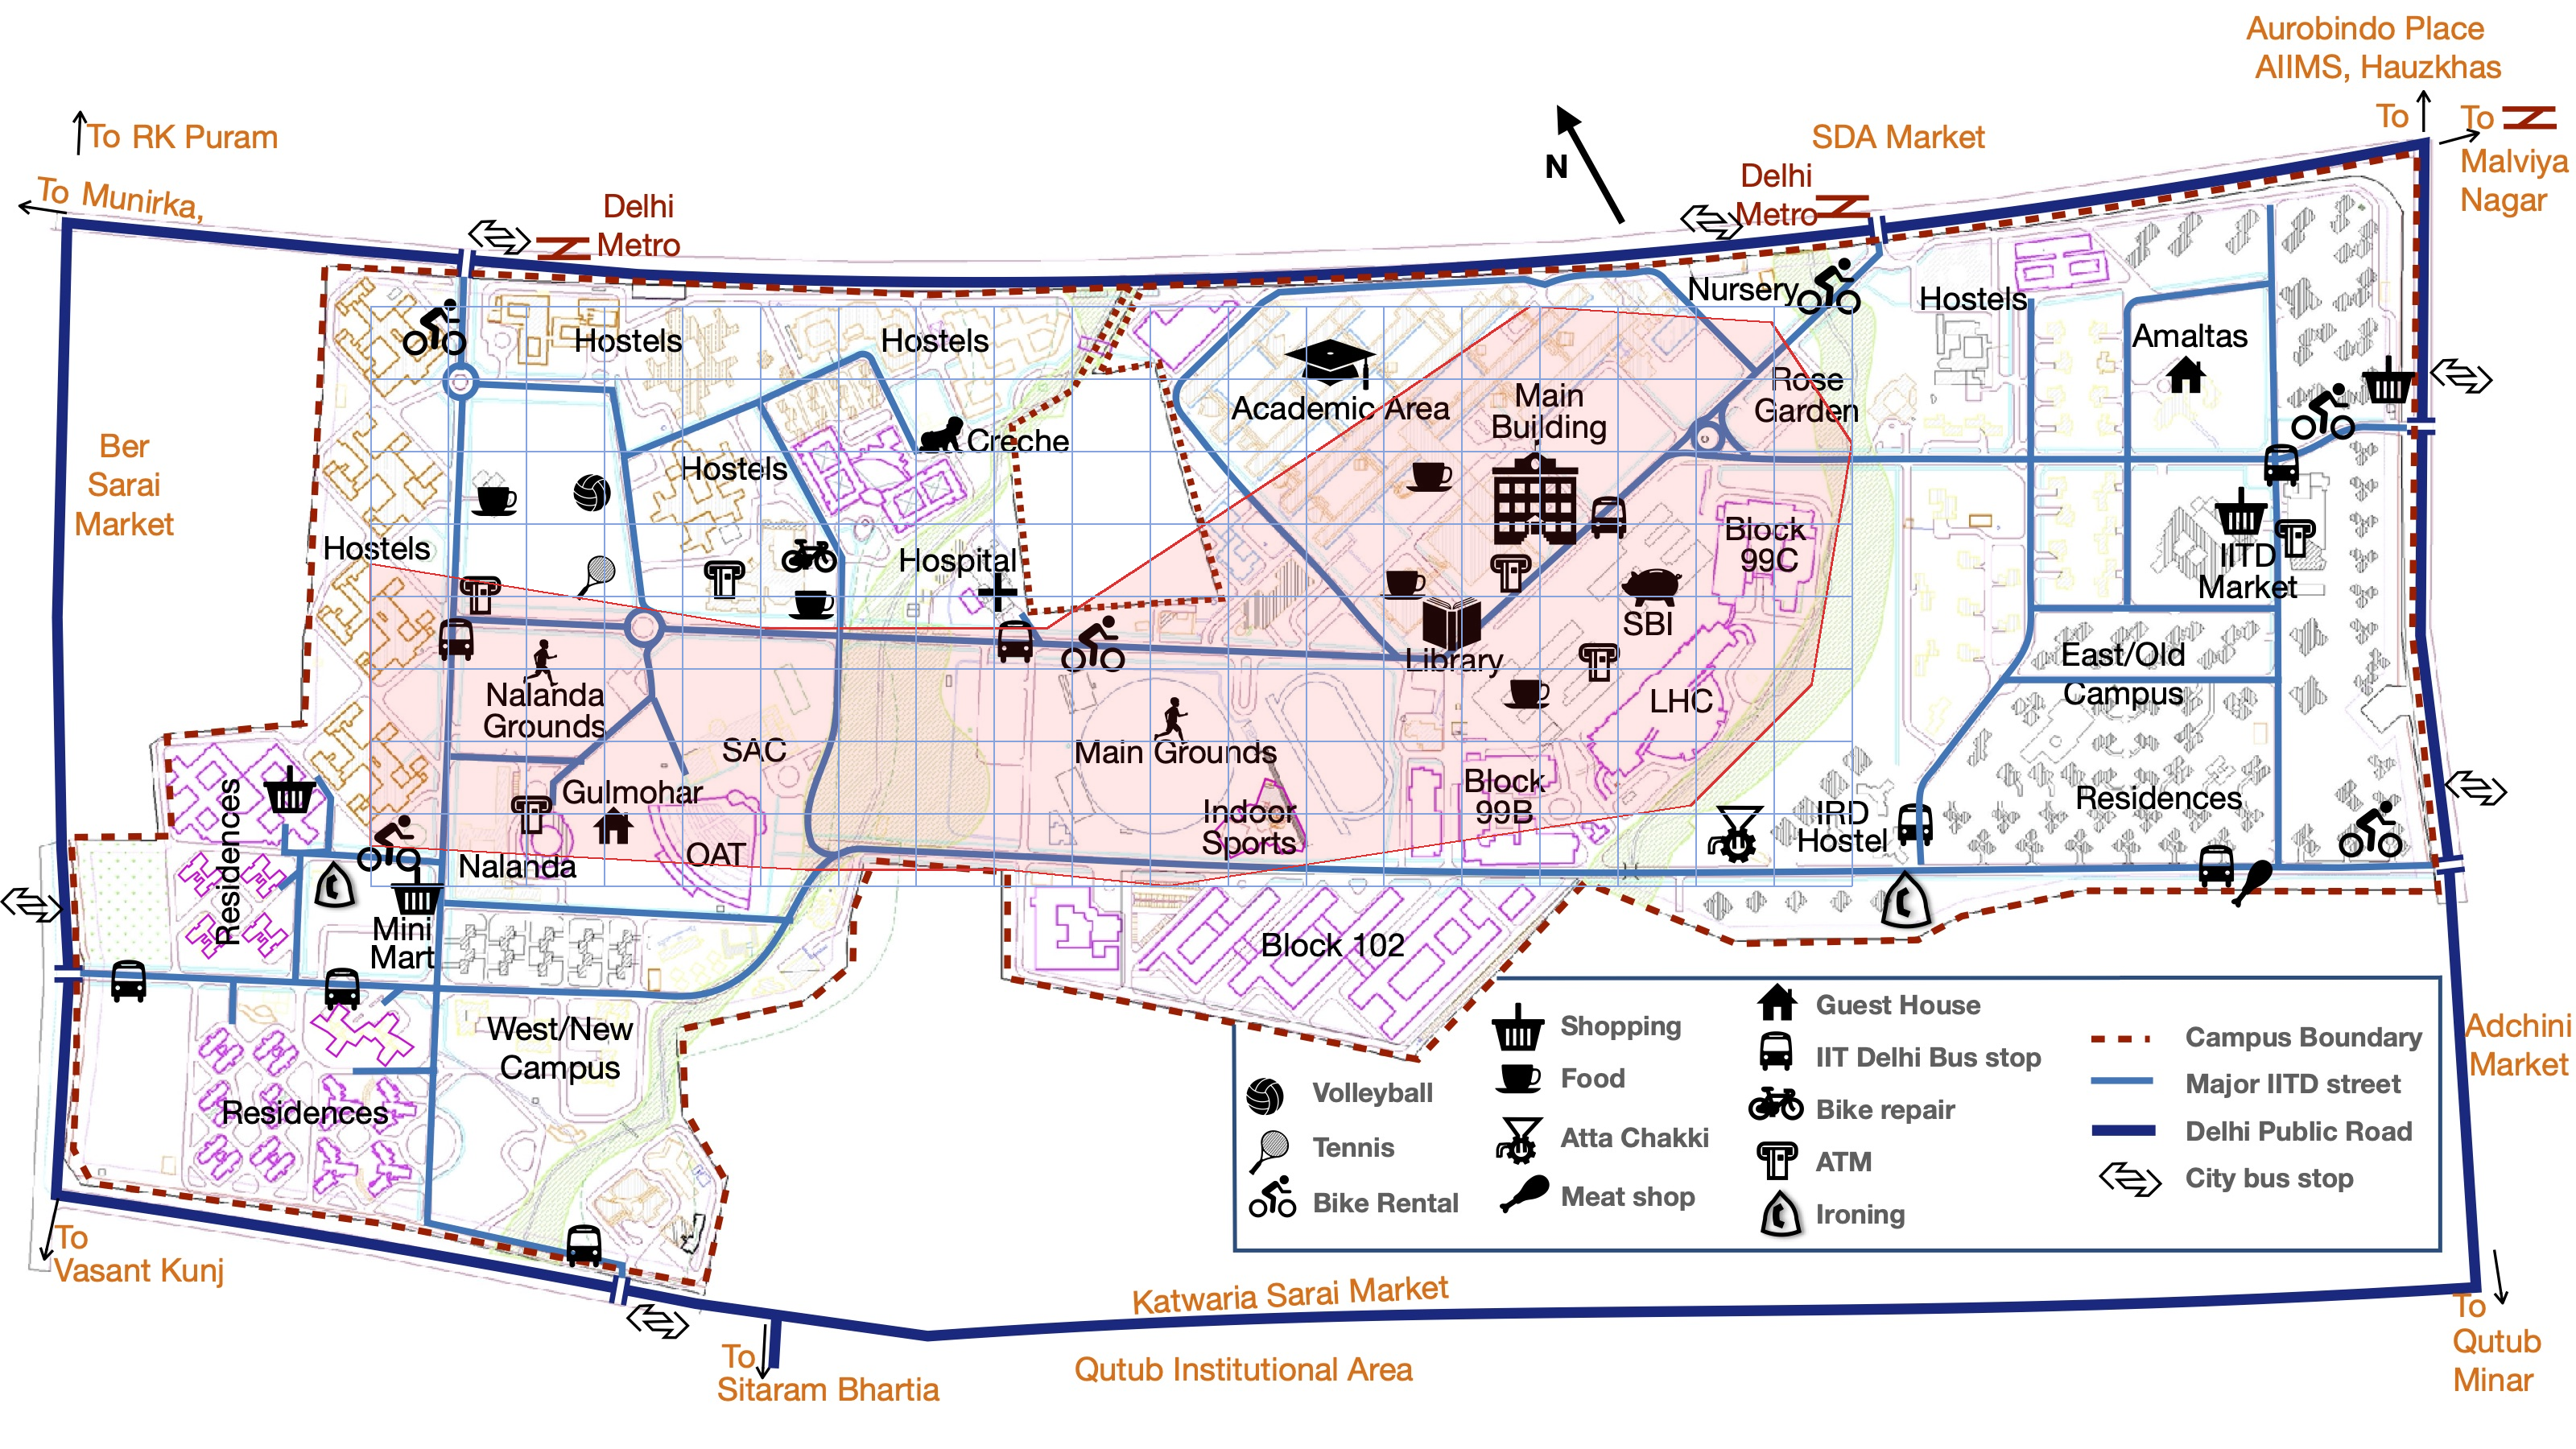
\includegraphics[width=\textwidth]{../Module_3_1/iitd_roi_grid_map.jpg}
        \end{column}
        \begin{column}{0.38\textwidth}
            \begin{block}{Spatial Analysis}
                \begin{itemize}
                    \item \textbf{Total ROI Area}: \textbf{82 acres} (26\% of Campus)
                    \item \textbf{Grid System}: \textbf{137 cells} (0.6 acres each)
                \end{itemize}
            \end{block}
            \begin{alertblock}{Zones}
                \begin{enumerate}
                    \item \textbf{West}: Nalanda, SAC (Events)
                    \item \textbf{East}: Sports, Academic, Rose Garden (Main)
                    \item \textbf{Corridor}: Connecting path
                \end{enumerate}
            \end{alertblock}
        \end{column}
    \end{columns}
\end{frame}

\begin{frame}{ROI Metrics Breakdown}
    \begin{table}
        \caption{Zonal Breakdown of Rendezvous ROI}
        \centering
        \begin{tabular}{llcc}
            \toprule
            \textbf{Zone} & \textbf{Description} & \textbf{Area (ac)} & \textbf{Type} \\ \midrule
            West & Nalanda, SAC, OAT & 25 & Venue \\
            East & Sports, Academic, Rose Garden & 52 & Main Zone \\
            Circulation & Internal Corridors & 5 & Transit \\
            \midrule
            \textbf{Total} & \textbf{Consolidated Region} & \textbf{82} & --- \\
            \bottomrule
        \end{tabular}
    \end{table}
    
    \vspace{0.2cm}
    \begin{itemize}
        \item \textbf{Why this region?} These areas concentrate 90\% of festival footfall.
        \item \textbf{Grid Purpose}: Enables precise "Dustbin Placement" (Module 3.2).
    \end{itemize}
\end{frame}

%%%%%%%%%%%%%%%%%%%%%%%%%%%%%%%%%%%%%%%%%%%%%%%%%%%%%%%%%%%%%%%%%
\section{Results \& Optimality}
%%%%%%%%%%%%%%%%%%%%%%%%%%%%%%%%%%%%%%%%%%%%%%%%%%%%%%%%%%%%%%%%%

\begin{frame}{Preliminary Optimization Results}
    \begin{block}{The "Optimal" Stall Count}
        For $N = 40,000$ (daily attendees), differentiating $E$ w.r.t $S$:
        $$ S^* \approx N \sqrt{\frac{\gamma_{NS}}{\alpha_2}} $$
        
        Using our parameters:
        $$ S^* \approx 40000 \sqrt{\frac{0.0005}{18}} \approx \textbf{210 Stalls} $$
    \end{block}

    \begin{itemize}
        \item \textbf{Current State}: Typically $\sim$100 stalls.
        \item \textbf{Insight}: We are currently \textbf{under-provisioned}.
        \item \textbf{Consequence}: The Congestion Penalty ($\gamma_{NS} N^2/S$) is dominating the environmental load (excess littering due to long queues).
        \item \textbf{Recommendation}: Increasing infrastructure to $\sim$210 stalls will actually \textit{reduce} total environmental impact by mitigating waste leakage.
    \end{itemize}
\end{frame}

\begin{frame}{Conclusion \& Next Steps}
    \begin{columns}[T]
        \begin{column}{0.48\textwidth}
            \begin{exampleblock}{Module 3.1 Summary}
                \begin{enumerate}
                    \item Built a comprehensive Environ-Load Model ($E$).
                    \item Identified "Congestion" as the silent killer of sustainability.
                    \item Mapped the exact festival ROI (82 acres).
                \end{enumerate}
            \end{exampleblock}
        \end{column}

        \begin{column}{0.48\textwidth}
            \begin{block}{Path Forward}
                \begin{itemize}
                    \item \textbf{Module 3.2}: Place dustbins optimally within the 137-cell grid.
                    \item \textbf{Module 3.3}: Route planning for waste collection vehicles.
                    \item \textbf{Module 3.4}: Water refill station coverage.
                \end{itemize}
            \end{block}
        \end{column}
    \end{columns}

    \vspace{0.5cm}
    \centering
    \textit{Optimization is the key to a Greener Rendezvous!}
\end{frame}

% --- FINAL SLIDE ---
\begin{frame}[plain]
    \vfill
    \begin{center}
        {\Huge \textcolor{DarkNavy}{Thank You}}
        
        \vspace{1cm}
        {\Large \textbf{Target: Zero Waste Rendezvous}}
        
        \vspace{1cm}
        \small Project 3: Sustainable Festival Challenge
    \end{center}
    \vfill
\end{frame}

\end{document}
